%!TEX root = ../six_pole.tex
% Тип документа
\documentclass[a4paper,12pt]{extarticle}

% Шрифты, кодировки, символьные таблицы, переносы
% \usepackage{cmap}
% \usepackage[T2A]{fontenc}
\usepackage[utf8]{inputenc}
\usepackage[russian]{babel}
% Это пакет -- хитрый пакет, он нужен но не нужен
\usepackage[mode=buildnew]{standalone}

\usepackage
	{
		% Дополнения Американского математического общества (AMS)
		amssymb,
		amsfonts,
		amsmath,
		amsthm,
		% Пакет для физических текстов
		physics,
		% misccorr,
		% 
		% Графики и рисунки
		wrapfig,
		graphicx,
		subcaption,
		float,
		tikz,
		tikz-3dplot,
		caption,
		csvsimple,
		color,
		booktabs,
		geometry,
		% 
		% Таблицы, списки
		makecell,
		multirow,
		indentfirst,
		%
		% Интегралы и прочие обозначения
		ulem,
		esint,
		esdiff,
		% 
		% Колонтитулы
		fancyhdr,
	}  
\usepackage{pgfplots,pgfplotstable,booktabs,colortbl}
\usepackage{xcolor}
\usepackage{hyperref}

 % Цвета для гиперссылок
\definecolor{linkcolor}{HTML}{000000} % цвет ссылок
\definecolor{urlcolor}{HTML}{799B03} % цвет гиперссылок
 
\hypersetup{pdfstartview=FitH,linkcolor=linkcolor,urlcolor=urlcolor, colorlinks=true}
\hypersetup{pageanchor=false}
% Увеличенный межстрочный интервал, французские пробелы
\linespread{1.3} 
\frenchspacing 

 
% \usetikzlibrary
% 	{
% 		decorations.pathreplacing,
% 		decorations.pathmorphing,
% 		patterns,
% 		calc,
% 		scopes,
% 		arrows,
% 		fadings,
% 		through,
% 		shapes.misc,
% 		arrows.meta,
% 		3d,
% 		quotes,
% 		angles,
% 		babel
% 	}
% Среднее <#1>
\newcommand{\mean}[1]{\langle#1\rangle}
% const прямым шрифтом
\newcommand\ct[1]{\text{\rmfamily\upshape #1}}
\newcommand*{\const}{\ct{const}}
\usepackage{array}
\usepackage{pstool}

\geometry		
	{
		left			=	2cm,
		right 			=	2cm,
		top 			=	2.5cm,
		bottom 			=	2.5cm,
		bindingoffset	=	0cm
	}

%%%%%%%%%%%%%%%%%%%%%%%%%%%%%%%%%%%%%%%%%%%%%%%%%%%%%%%%%%%%%%%%%%%%%%%%%%%%%%%
	%применим колонтитул к стилю страницы
\pagestyle{fancy} 
	%очистим "шапку" страницы
% \fancyhead{} 
	%слева сверху на четных и справа на нечетных
\fancyhead[R]{}%\labauthors 
	%справа сверху на четных и слева на нечетных
% \fancyhead[L]{Отчёт по лабораторной работе №\labnumber}
\fancyhead[L]{\labtheme} 
	%очистим "подвал" страницы
% \fancyfoot{} 
	% номер страницы в нижнем колинтуле в центре
\fancyfoot[C]{\thepage} 

%%%%%%%%%%%%%%%%%%%%%%%%%%%%%%%%%%%%%%%%%%%%%%%%%%%%%%%%%%%%%%%%%%%%%%%%%%%%%%%

\renewcommand{\contentsname}{Оглавление}
\usepackage{tocloft}
\usepackage{secdot}
\sectiondot{subsection}
\usepackage{gensymb}
\usepackage{textcomp}
\usepackage{pythontex}

\begin{document}
\def\labauthors{Карусевич А.А, Понур К.А.}
\def\labgroup{430}
\def\department{Кафедра электродинамики}
\def\labnumber{1}
\def\labtheme{Экспериментальное определение элементов матрицы рассеяния шестиполюсников}

\renewcommand{\Re}{\operatorname{Re}}
\renewcommand{\Im}{\operatorname{Im}}
\renewcommand{\phi}{\varphi}
\renewcommand{\hat}{\widehat}

\begin{titlepage}

\begin{center}

{\small\textsc{Нижегородский государственный университет имени Н.\,И. Лобачевского}}
\vskip 1pt \hrule \vskip 3pt
{\small\textsc{Радиофизический факультет}}



\vfill
{\Large {\department}}

{\Large Отчет по лабораторной работе №\labnumber\vskip 12pt\bfseries \labtheme}
	
\end{center}

\vfill
	
\begin{flushright}
	{Выполнили студенты \labgroup\ группы\\ \labauthors}%\vskip 12pt Принял:\\ Менсов С.\,Н.}
\end{flushright}
	
\vfill
	
\begin{center}
	Нижний Новгород, \the\year
\end{center}

\end{titlepage}


\tableofcontents
\newpage


\section*{Введение}
\addcontentsline{toc}{section}{Введение}
\label{sec:input}

В данной работе изучаются с помощью матричного анализа волноводные узлы -- шестиполюсники. У них с помощью измерительной линии измеряются величины, позволяющие рассчитать коэффициенты матрицы рассеяния шестиполюсников $S_{km}$. 

На основе рассчитанной матрицы рассеяния $S$ конкретного шестиполюсников можно попытаться решить обратную задачу: сделать на основе полученных данных предположение о возможных конструктивных вариантах волноводных узлов, находящихся внутри шестиполюсников.

\section{Теоретические сведения}
\subsection{Матрица рассеяния шестиполюсника}

Рассмотрим трехплечий волноводный узел (шестиполюсник), изображенный на рис. 1. В каждом плече выберем \textbf{плоскость отсчета} (сечение), в котором будем находить отношения амплитуд полей отраженной и падающей волн.

\begin{figure}[h!]
	\centering
	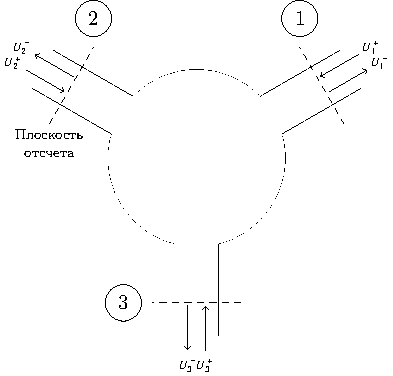
\includegraphics[scale=1.5]{ris/ris1}
	% \includegraphics[scale=1.5]{example-image-a}
	\caption{Схема трехплечего узла (шестиполюсника)}
	\label{fig:figure1}
\end{figure}

Обозначим комплексные амплитуды полей входящих (падающих) в узел волн через $U_m^+$, а амплитуды выходящих (отраженных) волн через $U_k^-$. 
Величины $U_k^-$ зависят от амплитуд и фаз полей волн, входящих во все плечи узла, причем эти зависимости являются линейными в силу линейности уравнений Максвелла (предполагается, что нелинейных элементов в узле нет). 
Связь между амплитудами полей в плечах узла записывается в виде:
\begin{equation}
	\begin{array} { l } { U _ { 1 } ^ { - } = S _ { 11 } U _ { 1 } ^ { + } + S _ { 12 } U _ { 2 } ^ { + } + S _ { 13 } U _ { 3 } ^ { + } } \\ { U _ { 2 } ^ { - } = S _ { 21 } U _ { 1 } ^ { + } + S _ { 22 } U _ { 2 } ^ { + } + S _ { 23 } U _ { 3 } ^ { + } } \\ { U _ { 3 } ^ { - } = S _ { 31 } U _ { 1 } ^ { + } + S _ { 32 } U _ { 2 } ^ { + } + S _ { 33 } U _ { 3 } ^ { + } } \end{array}
\end{equation}
где $S_{km}$ ---  комплексные коэффициенты, характеризующие волноводный узел. 
Их физический смысл очевиден для случая, когда источник включен только в $m$-е плечо ($U_m^+\ne0$), а все остальные плечи нагружены на согласованные нагрузки, и входящие в узел волны в них отсутствуют ($U_i^+=0$, если $i\ne m$). 

В этом случае диагональный элемент $S_{mm}$ представляет собой отношение комплексной амплитуды волны, отраженной от $n$-го входа, к амплитуде волны, поступающей на этот вход:

\begin{equation}
	S _ { m m } = U _ { m } / U _ { m } ^ { + }
\end{equation}
т.е. является коэффициентом отражения волны в $m$-ом плече. Недиагональный элемент $S_{km}$ определяет вклад волны, падающей на $m$-ый вход, в волну, выходящую из $k$-го входа:
\begin{equation}
	S _ { k m } = U _ { k } / U _ { m } ^ { + }
\end{equation}
т.е. является коэффициентом передачи волны из $m$-го плеча в $k$-ое плечо. Систему уравнений (1) удобно записать в матричной форме
\begin{equation}
	\left( \begin{array} { c } { U _ { 1 } ^ { - } } \\ { U _ { 2 } ^ { - } } \\ { U _ { 3 } ^ { - } } \end{array} \right) = \hat { S } \left( \begin{array} { l } { U _ { 1 } ^ { + } } \\ { U _ { 2 } ^ { + } } \\ { U _ { 3 } ^ { + } } \end{array} \right)
\end{equation}
где
\begin{equation}
	\hat { \mathbf { S } } = \left( \begin{array} { c c c } { S _ { 11 } } & { S _ { 12 } } & { S _ { 13 } } \\ { S _ { 21 } } & { S _ { 22 } } & { S _ { 23 } } \\ { S _ { 31 } } & { S _ { 32 } } & { S _ { 33 } } \end{array} \right)
\end{equation}
--- матрица рассеяния, или $S$-матрица (от англ. scattering -- рассеяние).

Из определения элементов матрицы рассеяния (2), (3) следует, что для пассивных узлов, не обладающих свойством усиления мощности, модули коэффициентов передачи и отражения не могут превышать единицы.
\subsection{Отражение свойств шестиполюсника в матрице рассеяния}


\paragraph{Взаимный узел.} Волноводные узлы, в которых отсутствуют элементы с гиротропными свойствами (например, намагниченный феррит), являются взаимными устройствами. Их матрицы рассеяния симметричны относительно главной диагонали

\begin{equation}
	S_{mk}=S_{km}
\end{equation}

Верно и обратное утверждение: если волноводное устройство описывается симметричной матрицей рассеяния, то оно является взаимным.

\paragraph{Волноводное устройство без потерь.} Покажем, что матрица рассеяния волноводного устройства без потерь является унитарной, т.е.

\begin{equation}
	\mathbf { S } ^ { \mathrm { T } } \mathbf { S } ^ { * } = \hat { \mathbf { I } }
\end{equation}

Здесь символы <<$\mathrm { T }$>> и <<$*$>> обозначают операции транспонирования и комплексного сопряжения соответственно. Выражение (6) можно также записать в виде

\begin{equation}
	\sum _ { m = 1 } ^ { N } S _ { l m } ^ { \mathrm { T } } S _ { m k } ^ { * } = \delta _ { l k }
\end{equation}
где $N$ -- число плеч волноводного узла, $\delta_{ik}$ -- индекс Кронекера.

Если в узле отсутствуют источники поля и, кроме того, потерь в узле нет (т.е. элементы узла являются реактивными), то согласно закону сохранения энергии суммарная мощность выходящих волн равна суммарной мощности падающих волн:

\begin{equation}
	\sum _ { m = 1 } ^ { N } \left| U _ { m } ^ { - } \right| ^ { 2 } = \sum _ { m = 1 } ^ { N } \left| U _ { m } ^ { + } \right| ^ { 2 }
\end{equation}

Правую часть выражения (8) перепишем следующим образом:

\begin{equation}
	\sum _ { m = 1 } ^ { N } \left| U _ { m } ^ { + } \right| ^ { 2 } = \sum _ { m = 1 } ^ { N } \left( U _ { m } ^ { + } \right) ^ { * } U _ { m } ^ { + } = \sum _ { m = 1 } ^ { N } \sum _ { k = 1 } ^ { N } \sum _ { l = 1 } ^ { N } \delta _ { m k } \delta _ { m l } \left( U _ { k } ^ { + } \right) ^ { * } U _ { l } ^ { + }
\end{equation}

В свою очередь, левая часть равенства (8) с учетом (1) примет вид: 

\begin{equation}
	\sum _ { m = 1 } ^ { N } \left| U _ { m } ^ { - } \right| ^ { 2 } = \sum _ { m = 1 } ^ { N } \left( U _ { m } ^ { - } \right) ^ { * } U _ { m } ^ { - } = \sum _ { m = 1 } ^ { N } \sum _ { k = 1 } ^ { N } \sum _ { l = 1 } ^ { N } S _ { m k } ^ { * } S _ { m l } \left( U _ { k } ^ { + } \right) ^ { * } U _ { l } ^ { + }
\end{equation}


Тогда из (8) получим

\begin{equation}
	\sum _ { k = 1 } ^ { N } \sum _ { l = 1 } ^ { N } \left\{ \sum _ { m = 1 } ^ { N } \left[ S _ { m l } S _ { m k } ^ { * } - \delta _ { m l } \delta _ { m k } \right] \right\} \left( U _ { k } ^ { + } \right) ^ { * } U _ { l } ^ { + } = 0
\end{equation}

Поскольку $U_k^+, U_l^+$ -- произвольны, выражение в фигурной скобке равно нулю и, следовательно, с учетом

\begin{equation}
	\sum _ { m = 1 } ^ { N } \delta _ { m l } \delta _ { m k } = \delta _ { l k }
\end{equation}
справедливо соотношение
\begin{equation}
	\sum _ { m = 1 } ^ { N } S _ { m l } S _ { m k } ^ { * } = \delta _ { l k }
\end{equation}	

Принимая во внимание, что $S _ { m l } = S _ { l m } ^ { \mathrm { T } }$, приходим к выражению (7). 
Таким образом, доказано, что матрицы рассеяния устройств без потерь унитарны.



Для взаимных волноводных устройств матрица рассеяния является симметричной: $\hat { \mathbf { S } } ^ { \mathrm { T } } = \hat { \mathbf { S } }$. В этом случае из (6) получаем, что для взаимных устройств без потерь

\begin{equation}
	\hat { \mathbf { S } } \hat { \mathbf { S } } ^ { * } = \hat { \mathbf { I } }
\end{equation}

Из формулировки унитарности, представленной в виде (9), следует, что 

\begin{equation}
	\sum _ { m = 1 } ^ { N } S _ { m k } S _ { m k } ^ { * } = \sum _ { m = 1 } ^ { N } \left| S _ { m k } \right| ^ { 2 } = 1
\end{equation}
т.е. сумма квадратов модулей всех матричных элементов любого столбца матрицы рассеяния узла без потерь равна единице. 

Если узел взаимный, то и сумма квадратов модулей всех матричных элементов любой строки также равна единице. 
Кроме того, из (9) следует, что для любой пары столбцов сумма (по строкам) произведений каждого матричного элемента из одного столбца на комплексно сопряженный элемент из той же строки другого столбца равна нулю

\begin{equation}
	\sum _ { m = 1 } ^ { N } S _ { m l } S _ { m k } ^ { * } = 0 , \quad k \neq l
\end{equation}

Очевидно, что для взаимной системы аналогичное соотношение имеет место и для элементов любой пары строк матрицы рассеяния.

\paragraph{Смещение плоскости отсчета.} Предположим, что известна матрица рассеяния при некотором положении плоскости отсчета $z = 0$ в $m$-ом плече узла. При смещении этого сечения на расстояние $l_m$ в направлении распространения падающей волны (по направлению к узлу) новое значение комплексной амплитуды будет

\begin{equation}
	\left( U _ { m } ^ { + } \right) ^ { \prime } = U _ { m } ^ { + } e ^ { - i h _ { m } l _ { m } }
\end{equation}

где $h_m$ -- постоянная распространения волны в $m$-ом плече. Соответственно амплитуда отраженной волны

\begin{equation}
	\left( U _ { m } ^ { - } \right) ^ { \prime } = U _ { m } ^ { - } e ^ { i h _ { m } l _ { m } }
\end{equation}

Если перемещать плоскость отсчета в положительном направлении в первом плече на $l_1$, во втором на $l_2$ и т.д., то волноводный узел будет характеризоваться новой матрицей рассеяния $\hat { \mathbf { S } } ^ { \prime }$, которая связывает новые амплитуды $\left( \mathbf { U } ^ { - } \right) ^ { \prime } = \hat { \mathbf { S } } ^ { \prime } \left( \mathbf { U } ^ { + } \right) ^ { \prime }$. При этом отраженную волну в $m$-ом плече можно записать в виде

\begin{equation}
	(U_m^-)'=S_{m1}'(U_1^+)'+S_{m2}'(U_2^+)'+\ldots+S_{mn}'(U_n^+)'.
\end{equation}

Сравнивая (15) с (1) и учитывая (13), (14), а также произвольность амплитуд, имеем

\begin{equation}
	\begin{array} { l } { S _ { m k } ^ { \prime } = S _ { m k } e ^ { i \left( h _ { m } l _ { m } + h _ { k } l _ { k } \right) } } \\ { S _ { m m } ^ { \prime } = S _ { m m } e ^ { i 2 h _ { m } l _ { m } } } \end{array}
\end{equation}

Таким образом, изменение плоскости отсчета приводит лишь к изменению фазы коэффициентов матрицы рассеяния, не меняя их абсолютного значения. Поскольку выбор плоскостей отсчета произволен, преобразование (16) позволяет в некоторых случаях упростить матричные элементы, сделав их действительными числами.

Перечисленные выше свойства матриц рассеяния используются при расчетах волноводных устройств.

\subsection{Определение коэффициента отражения от нагрузки}


Напряжение в линии передачи (рис. П.1) с волновым сопротивлением $Z_B$ и сопротивлением нагрузки $Z_H$ представляет собой сумму падающей и отраженной волн

\begin{equation}
	U=U_\text{пад}+U_\text{отр}
\end{equation}

На конце линии, где включено сопротивление нагрузки $Z_H$ (рис. П.1), напряжение равно

\begin{equation}
	U_H=U=U_\text{пад,H}+U_\text{отр,H}=U_\text{пад,H}(1+\Gamma),
\end{equation}

где комплексная величина

\begin{equation}
	\Gamma=\left(\frac{U_\text{пад}}{U_\text{отр}}\right)_H= | \Gamma | e ^ { i \varphi _ { \mathrm { H } } }
\end{equation}

называется коэффициентом отражения.

\begin{figure}[h!]
	\centering
	% 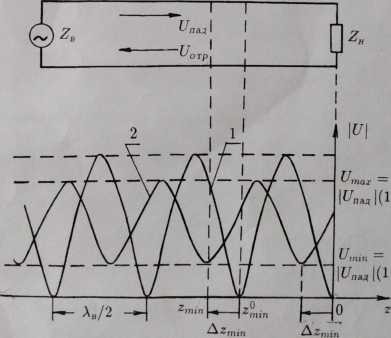
\includegraphics{img/2.jpg}
	\caption{Распределение модуля напряжения вдоль линии: 1 -- режим короткого замыкания ($Z_H=0$); 2 -- произвольный импеданс на конце линии ($Z_H\ne0$)}
	\label{fig:p1}
\end{figure}
В формуле (П.З)
\begin{equation}
	|\Gamma|=\left|\frac{U_\text{пад,H}}{U_\text{отр,H}}\right|=\left|\frac{U_\text{пад}}{U_\text{отр}}\right|,
\end{equation}
-- модуль коэффициента отражения, $\phi_H$ -- фаза коэффициента отражения в сечении нагрузки. Располагая начало координат $(z = 0)$ в плоскости нагрузки (рис. П.1), в произвольном сечении $z$ линии имеем
\begin{gather}
	U=U_\text{пад,H}e^{-ihz}+U_\text{отр,H}e^{ihz}=
		=U_\text{пад}(1+\Gamma e^{i2hz})=
		=U_\text{пад}(1+|\Gamma|e^{i\psi}),
\end{gather}
где
\begin{equation}
	\psi=\phi_H+2hz
\end{equation}
--- фаза коэффициента отражения в сечении 2, h -- постоянная распространения волны в линии.

Режим работы линии передачи удобно характеризовать коэффициентом стоячей волны К (КСВ), равным отношению максимального напряжения в линии к ее минимальному значению
\begin{equation}
	\mathrm { K } = \frac { | U | _ { \max } } { | U | _ { \min } }
\end{equation}
Иногда используется и обратная величина -- коэффициент бегущей волны (КБВ). В максимуме стоячей волны напряжения в падающей и отраженной волнах синфазны:
\begin{equation}
	|U|_{max}=|U_\text{пад}|+|U_\text{отр}|=|U_\text{пад}|(1+|\Gamma|),
\end{equation}
в минимуме -- противофазны:
\begin{equation}
	|U|_{min}=|U_\text{пад}|-|U_\text{отр}|=|U_\text{пад}|(1-|\Gamma|),
\end{equation}
Тогда
\begin{equation}
	\mathrm { K } = \frac { 1 + | \Gamma | } { 1 - | \Gamma | },
\end{equation}
откуда получим
\begin{equation}
	| \Gamma | = \frac { K - 1 } { K + 1 }
\end{equation}

Нетрудно убедиться в том, что К изменяется от единицы до бесконечности, причем режиму согласования, когда $Z_H = Z_B$, соответствует значение $\mathrm{К}=1$, а режиму короткого замыкания (или холостого хода), а также любой реактивной нагрузке -- $\mathrm{К}=\infty$.

Измерение К может быть произведено путем перемещения вдоль измерительной линии (ИЛ) прибора, показания которого связаны с высокочастотным напряжением в данном сечении линии. 
В случае коаксиальных и волноводных систем ИЛ снабжены зондом штыревого типа, расположенным вдоль силовых линий электрического поля и перемещающимся вдоль продольной щели. 
Схема ИЛ изображена на рис. П.2.
\begin{figure}[h!]
	\centering
	% 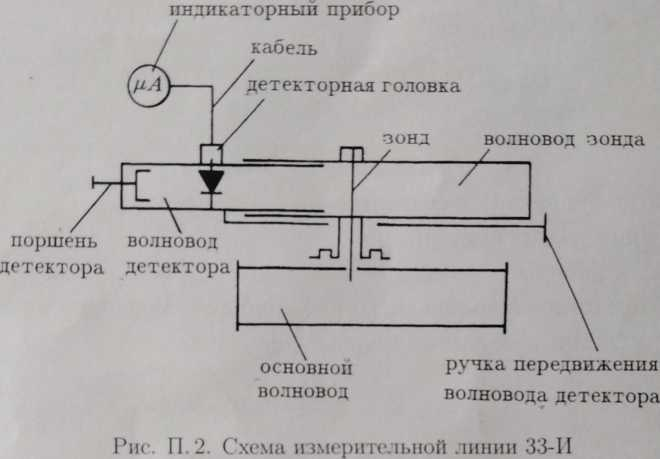
\includegraphics{img/3.jpg}
	\caption{Схема измерительной линии 33-И}
	\label{fig:figure1}
\end{figure}

Основной волновод измерительной линии включен в тракт испытуемой волноводной системы. 
При перемещении вдоль щели основного волновода зонд ответвляет часть электромагнитной энергии. 
Для детектирования СВЧ сигнала зонда в ИЛ обычно применяют кристаллические детекторы (СВЧ диоды). 
При этом зависимость между током детектора $I$ и приложенным высокочастотным напряжением $|U|$ является нелинейной.

Из теории детектирования известно, что при малых значениях переменного напряжения детектор имеет характеристику $I=f(|U|)$, близкую к квадратичной. В этом случае ток детектора
\begin{equation}
	I=\alpha|U|^2,
\end{equation}
где $\alpha$ --- параметр, зависящий от свойств детектора.

В максимуме и в минимуме распределения поля в линии имеем
\begin{equation}
	I _ { \max } = \alpha | U | _ { \min x } ^ { 2 } , \quad I _ { \min } = \alpha | U | _ { \min } ^ { 2 }
\end{equation}
откуда
\begin{equation}
	\mathrm { K } = \sqrt { \frac { I _ { \mathrm { max } } } { I _ { \mathrm { min } } } }
\end{equation}

Опыт показывает, что для современных стандартных кристаллических детекторов выражение (П.10) оказывается справедливым при выпрямленных токах менее $\sim20$ мкА.

Величину фазы коэффициента отражения в сечении $z$ ($z<0$) --- $\psi=\phi_H+2hz$ можно определить, например, зная положения точек $z_{min}$ минимального значения напряжения. Из (П.6) нетрудно видеть, что
\begin{equation}
	\psi \left( z _ { \min } \right) = ( 2 n - 1 ) \pi = \varphi _ { \mathrm { H } } + 2 h z _ { \min }
\end{equation}
и при $n = 0$ имеем

\begin{equation}
	\varphi _ { \mathrm { H } } = - 2 h z _ { \mathrm { min } } - \pi
\end{equation}

Таким образом, для определения фазы коэффициента отражения достаточно определить положение минимума напряжения в ИЛ\footnote{При характеристике детектора, близкой к квадратичной, минимум тока детектора никогда не бывает четко выраженным, особенно при небольших К. Для повышения точности отсчета положений минимумов $z_{\min}$ применяют метод <<вилки>>, состоящий в определении двух положений зонда $z_1$ и $z_2$ при одинаковых показаниях индикатора и вычислении $z_{\min}$ по формуле $z_{\min}=(z_1+z_2)/2$.} относительно плоскости присоединения нагрузки. 
%
Для этого необходимо найти т.н. \textbf{условный конец линии} -- сечение волновода, соответствующее минимуму напряжения при коротком замыкании линии ($z^0_{min}$ на рис. П.1), и заменить в (П.13) величину $Z_{min}$ на $(z_{min}-z_{min}^0)$. 
Расстояние от условного конца линии $z^0_{min}$ до ближайшего минимума напряжения $z_{min}$ \textbf{со стороны генератора} при включенной нагрузке обозначим через 
$\Delta z _ { \min } \equiv z _ { \min } ^ { 0 } - z _ { \min } = \left| z _ { \min } - z _ { \min } ^ { 0 } \right| =- \left( z _ { \min } - z _ { \min } ^ { 0 } \right)$

Тогда, согласно (П.13),  $\varphi _ { \mathrm { H } } = 2 h \Delta z _ { \mathrm { min } } - \pi$ и фаза коэффициента отражения (с учетом выражения $h=2\pi/\lambda_B$) будет определяться формулой
\begin{equation}
	\varphi _ { \mathrm { H } } = 4 \pi \frac { \Delta z _ { \mathrm { min } } } { \lambda _ { \mathrm { B } } } - \pi
\end{equation}

\section{Эксперимент}

\subsection{Используемое оборудование}

Мы ознакомились с устройством и работой генератора Г4-225 и измерительной волноводной линией 33-И. Включили и подготовить к работе генератор. Выбранное значение несущей частоты генератора -- 8,5 ГГц. В ходе эксперимента мощность сигнала ослаблялась на $-3\ldots-6$ дБ.

\subsection{Фиксация условного конца линии. Длина волны в волноводе}

Закоротили с помощью короткозамыкателя (КЗ) измерительную линию, на конце которой  находилась скрутка волновода. Резонатор измерительной линии настроили на максимум показаний индикатора. Далее зонд измерительной линии установили в ближайший к концу линии узел стоячей волны. Координату узла $z^0_{min}=5.75$ см в дальнейшем принимаем за условный конец линии. Измеритли длину волны в волноводе $\lambda_B=5.45 $ см.

\subsection{Проверка согласованных нагрузок}

Присоединили к скрутке волновода на конце измерительной линии каждую из двух используемых при выполнении работы согласованных нагрузок. Определили коэффициенты отражения от них
\begin{equation}
	\centering
 	\Gamma_{H_1}=0.062, ~~~ \Gamma_{H_2}=0.048 
\end{equation}
Значения  $\Gamma_{H_{1,2}}$ определяют точность расчетов элементов матриц рассеяния шестиполюсников по формулам (18), (23)-(25).

\subsection{Измерение параметров шестиполюсников и расчет $S_{km}$}

Для каждого из предложенных шестиполюсников осуществить 6 описанных выше экспериментов. По данным измерений заполнить таблицу.

Элементы матрицы рассеяния $S_{km}$ рассчитываются по данным таблицы и формулам (18), (23)-(25). Вначале следует рассчитать диагональные элементы, а затем -- недиагональные. Результаты записываются в виде $S _ { k m } = \left| S _ { k m } \right| e ^ { i \varphi _ { k m } }$.

\subsubsection{Измерение диагональных элементов}
К плечу 1 (риc. За) через развязывающий аттенюатор (РА) и измерительную линию (ИЛ) подключается генератор электромагнитных  колебаний (Г), а плечи 2 и 3 соединяются согласованными нагрузками (Н). 
При этом в плечах 2 и 3 отраженные от нагрузок волны отсутствуют, т.е. $U _ { 2 } ^ { + } = U _ { 3 } ^ { + } = 0$.


Первое уравнение системы (1) принимает вид $U_1^-=S_{11}U_1^+$, или
\begin{equation}
	S _ { 11 } = U _ { 1 } ^ { - } / U _ { 1 } ^ { + }
\end{equation}
где $U _ { 1 } ^ { - }$ и $U _ { 1 } ^ { + }$ -- комплексные амплитуды отраженной и падающей волн на входе первого плеча шестиполюсника. Отношение этих величин, равное коэффициенту отражения 
\begin{equation}
	\Gamma _ { 11 } = S _ { 11 } = \left| \Gamma _ { 11 } \right| e ^ { i \varphi _ { 11 } }
\end{equation}
можно найти с помощью измерительной линии на основе обычной методики измерения коэффициента стоячей волны и определения положения минимума напряжения (см. Приложение). 
Присоединяя генератор по указанной на рис. За схеме поочередно к плечам 2 и 3, определяют элементы $S_{22}$ и $S_{33}$.

\begin{figure}[h!]
	\centering
	% 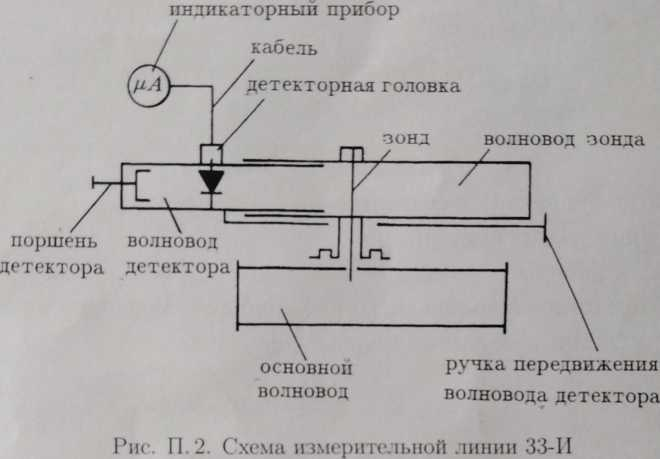
\includegraphics[]{img/3.jpg}
	\caption{Схема измерения элементов $S_{11}$ и $S_{12}$:  Г --- генератор Г4-225, РА  -- развязывающий аттенюатор, ИЛ - измерительная волноводная линия 33-И, СВ - скрутка волновода,  Н -- согласованная нагрузка, КЗ --- короткозамыкатель.}
	\label{fig:fig3}
\end{figure}



\subsubsection{Измерение недиагональных элементов}

Рассмотрим другой вариант, отличающийся от предыдущего тем. что плечо 2 короткозамкнуто (рис. 3 6). Теперь лишь $U_3^+=0$, и первые два уравнения системы (1) примут вид
\begin{equation}
	\begin{array} { l } { U _ { 1 } ^ { - } = S _ { 11 } U _ { 1 } ^ { + } + S _ { 12 } U _ { 2 } ^ { + } } \\ { U _ { 2 } ^ { - } = S _ { 21 } U _ { 1 } ^ { + } + S _ { 22 } U _ { 2 } ^ { + } } \end{array}
\end{equation}
Учтем, что в силу граничных условий в точке короткого замыкания амплитуды $U_2^+$ и $U_2^-$ удовлетворяют уравнению
\begin{equation}
	U _ { 2 } ^ { + } = - U _ { 2 } ^ { - }
\end{equation}
Подставляя (20) в (19), находим отношение амплитуд встречных волн в первом плече:
\begin{equation}
	\begin{array} { l } { \Gamma _ { 12 } = \frac { U _ { 1 } ^ { - } } { U _ { 1 } ^ { + } } = S _ { 11 } - S _ { 12 } \frac { U _ { 2 } ^ { - } } { U _ { 1 } ^ { + } } } \\ { \frac { U _ { 2 } ^ { - } } { U _ { 1 } ^ { + } } = \frac { S _ { 21 } } { 1 + S _ { 22 } } } \end{array}
\end{equation}
Подставляя выражение для $U_2^-/U_1^+$ в первое уравнение (21), найдем коэффициент отражения $\Gamma_{12}$ на входе первого плеча шестиполюсника, включенного по схеме, изображенной на рис. 3б:
\begin{equation}
	\Gamma _ { 12 } = S _ { 11 } - \frac { S _ { 12 } S _ { 21 } } { 1 + S _ { 22 } }
\end{equation}
Тогда для произведения недиагональных элементов матрицы рассеяния имеем
\begin{equation}
	S _ { 12 } S _ { 21 } = \left( 1 + S _ { 22 } \right) \left( S _ { 11 } - \Gamma _ { 12 } \right)
\end{equation}
Поскольку диагональные элементы $S_{mm}$ известны (из предыдущих экспериментов), а коэффициент отражения $\Gamma_{12}=|\Gamma_{12}|е^{i\phi_{12}}$ можно найти с помощью измерительной линии, то этот эксперимент дает возможность определить произведение $S_{12}S_{21}$.
При такой методике измерения невозможно определить отдельно элементы $S_{12}$ и $S_{21}$, однако, если шестиполюсник не содержит невзаимных элементов, то, согласно (5), $S_{12} = S_{21}$ и $S_{12}S_{21}=S_{12}^2$. 
Поэтому (возможно ошибка в знаке)
\begin{gather}
	S _ { 12 } = \sqrt { S _ { 12 } S _ { 21 } } = \nonumber \\= \left\{ \left[ \operatorname { Re } \left( S _ { 12 } S _ { 21 } \right) \right] ^ { 2 } + \left[ \operatorname { Im } \left( S _ { 12 } S _ { 21 } \right) \right] ^ { 2 } \right\} ^ { 1 / 4 } \exp \left[ \frac { 1 } { 2 } \operatorname { arctg } \frac { \operatorname { Im } \left( S _ { 12 } S _ { 21 } \right) } { \operatorname { Re } \left( S _ { 12 } S _ { 21 } \right) } \right]
\end{gather}

Аналогично, закорачивая плечо 3 и присоединяя согласованную нагрузку к плечу 2, найдем 
\begin{equation}
	S _ { 13 } S _ { 31 } = S _ { 13 } ^ { 2 } = \left( 1 + S _ { 33 } \right) \left( S _ { 11 } - \Gamma _ { 13 } \right)
\end{equation}
где  $\Gamma _ { 13 } = \left| \Gamma _ { 13 } \right| e ^ { i \varphi _ { 13 } }$ -- коэффициент отражения на входе первого плеча в данной схеме включения шестиполюсника.

Для определения произведения $S_{23}S_{32}=S_{23}^2$ генератор следует
присоединить к плечу 2, нагрузку -- к плечу 1, а плечо 3 закоротить.
Тогда
\begin{equation}
	S _ { 23 } ^ { 2 } = \left( 1 + S _ { 33 } \right) \left( S _ { 22 } - \Gamma _ { 23 } \right)
\end{equation}
где $\Gamma _ { 23 } = \left| \Gamma _ { 23 } \right| e ^ { i p _ { 23 } }$ коэффициент отражения на входе плеча 2.

Таким образом, шесть описанных выше экспериментов дают возможность полностью определить все параметры  шестиполюсника.
Если шестиполюсник содержит невзаимные элементы, для отыскания его параметров следует производить 9 независимых экспериментов, причем необходимо также иметь возможность измерения величины сигнала, прошедшего в данное плечо.


\begin{table}[h!]
	\caption{Измерения характеристик шестиполюсника №1}
	\label{tab:1}
	\vspace{1em}
	\centering
	%!TEX root = six_pole.tex

\begin{tabular}{|l|l|l|l|l|l|l|l|l|l|l|l|l|l}
\cline{1-13}
\multicolumn{1}{|c|}{\multirow{2}{*}{N}} & \multicolumn{1}{c|}{\multirow{2}{*}{$S_{km}$}} & \multicolumn{3}{c|}{$N_{}$} & \multicolumn{1}{c|}{\multirow{2}{*}{$I_{min}$}} & \multicolumn{1}{c|}{\multirow{2}{*}{$I_{max}$}} & \multicolumn{1}{c|}{\multirow{2}{*}{K}} & \multicolumn{1}{c|}{\multirow{2}{*}{|Г|}} & \multicolumn{1}{c|}{\multirow{2}{*}{$z_{min}$}} & \multicolumn{1}{c|}{\multirow{2}{*}{$\Delta z$}} & \multicolumn{1}{c|}{\multirow{2}{*}{$\varphi_n$}} & \multicolumn{1}{c|}{\multirow{2}{*}{$S_{km}$}} &  \\ \cline{3-5}
\multicolumn{1}{|c|}{}                   & \multicolumn{1}{c|}{}                          & 1      & 2       & 3      & \multicolumn{1}{c|}{}                           & \multicolumn{1}{c|}{}                           & \multicolumn{1}{c|}{}                   & \multicolumn{1}{c|}{}                     & \multicolumn{1}{c|}{}                           & \multicolumn{1}{c|}{}                            & \multicolumn{1}{c|}{}                             & \multicolumn{1}{c|}{}                          &  \\ \cline{1-13}
1                                        & S11                                            & Г      & Н       & Н      & 30                                              & 24                                              & 1.118                                   & 0.056                                     & 4.495                                           & -1.255                                           & -6.03532                                          & 0.056                                          &  \\ \cline{1-13}
2                                        & S12                                            & Г      & КЗ      & Н      & 29                                              & 24                                              & 1.099                                   & 0.047                                     & 4.415                                           & -1.335                                           & -6.21978                                          & 0.094                                          &  \\ \cline{1-13}
3                                        & S13                                            & Г      & Н       & КЗ     & 29                                              & 24                                              & 1.099                                   & 0.047                                     & 4.6                                             & -1.15                                            & -5.79321                                          & 0.317                                          &  \\ \cline{1-13}
4                                        & S22                                            & Н      & Г       & Н      & 30                                              & 23                                              & 1.142                                   & 0.066                                     & 4.85                                            & -0.9                                             & -5.21677                                          & 0.066                                          &  \\ \cline{1-13}
5                                        & S23                                            & Н      & Г       & КЗ     & 30                                              & 23                                              & 1.142                                   & 0.066                                     & 4.885                                           & -0.865                                           & -5.13607                                          & 0                                              &  \\ \cline{1-13}
6                                        & S33                                            & Н      & Н       & Г      & 88                                              & 1                                               & 9.38                                    & 0.807                                     & 4.545                                           & -1.205                                           & -5.92003                                          & 0.807                                          &  \\ \cline{1-13}
\end{tabular}

\end{table}


\begin{table}[h!]
	\caption{Измерения характеристик шестиполюсника №2}
	\label{tab:2}
	\vspace{1em}
	\centering
	%!TEX root = six_pole.tex
\begin{tabular}{|l|l|l|l|l|l|l|l|l|l|l|l|l|l}
\cline{1-13}
\multicolumn{1}{|c|}{\multirow{2}{*}{N}} & \multicolumn{1}{c|}{\multirow{2}{*}{$S_{km}$}} & \multicolumn{3}{c|}{$N_{}$} & \multicolumn{1}{c|}{\multirow{2}{*}{$I_{min}$}} & \multicolumn{1}{c|}{\multirow{2}{*}{$I_{max}$}} & \multicolumn{1}{c|}{\multirow{2}{*}{K}} & \multicolumn{1}{c|}{\multirow{2}{*}{|Г|}} & \multicolumn{1}{c|}{\multirow{2}{*}{$z_{min}$}} & \multicolumn{1}{c|}{\multirow{2}{*}{$\Delta z$}} & \multicolumn{1}{c|}{\multirow{2}{*}{$\varphi_n$}} & \multicolumn{1}{c|}{\multirow{2}{*}{$S_{km}$}} &  \\ \cline{3-5}
\multicolumn{1}{|c|}{}                   & \multicolumn{1}{c|}{}                          & 1      & 2       & 3      & \multicolumn{1}{c|}{}                           & \multicolumn{1}{c|}{}                           & \multicolumn{1}{c|}{}                   & \multicolumn{1}{c|}{}                     & \multicolumn{1}{c|}{}                           & \multicolumn{1}{c|}{}                            & \multicolumn{1}{c|}{}                             & \multicolumn{1}{c|}{}                          &  \\ \cline{1-13}
1                                        & S11                                            & Г      & Н       & Н      & 85                                              & 1                                               & 9.220                                   & 0.804                                     & 4.91                                            & -0.84                                            & -5.078                                            & 0.804                                          &  \\ \cline{1-13}
2                                        & S12                                            & Г      & КЗ      & Н      & 85                                              & 1                                               & 9.220                                   & 0.804                                     & 4.955                                           & -0.795                                           & -4.975                                            & 0.111                                          &  \\ \cline{1-13}
3                                        & S13                                            & Г      & Н       & КЗ     & 94                                              & 1                                               & 9.695                                   & 0.813                                     & 4.79                                            & -0.96                                            & -5.355                                            & 0.112                                          &  \\ \cline{1-13}
4                                        & S22                                            & Н      & Г       & Н      & 54                                              & 9                                               & 2.449                                   & 0.420                                     & 4.97                                            & -0.78                                            & -4.940                                            & 0.420                                          &  \\ \cline{1-13}
5                                        & S23                                            & Н      & Г       & КЗ     & 91                                              & 1                                               & 9.539                                   & 0.810                                     & 4.725                                           & -1.025                                           & -5.505                                            & 0.746                                          &  \\ \cline{1-13}
6                                        & S33                                            & Н      & Н       & Г      & 50                                              & 8                                               & 2.500                                   & 0.429                                     & 4.81                                            & -0.94                                            & -5.309                                            & 0.429                                          &  \\ \cline{1-13}
\end{tabular}

\end{table}


\begin{table}[h!]
	\caption{Измерения характеристик шестиполюсника №3}
	\label{tab:3}
	\vspace{1em}
	\centering
	%!TEX root = six_pole.tex

\begin{tabular}{|l|l|l|l|l|l|l|l|l|l|l|l|l|l}
\cline{1-13}
\multicolumn{1}{|c|}{\multirow{2}{*}{N}} & \multicolumn{1}{c|}{\multirow{2}{*}{$S_{km}$}} & \multicolumn{3}{c|}{$N_{}$} & \multicolumn{1}{c|}{\multirow{2}{*}{$I_{min}$}} & \multicolumn{1}{c|}{\multirow{2}{*}{$I_{max}$}} & \multicolumn{1}{c|}{\multirow{2}{*}{K}} & \multicolumn{1}{c|}{\multirow{2}{*}{|Г|}} & \multicolumn{1}{c|}{\multirow{2}{*}{$z_{min}$}} & \multicolumn{1}{c|}{\multirow{2}{*}{$\Delta z$}} & \multicolumn{1}{c|}{\multirow{2}{*}{$\varphi_n$}} & \multicolumn{1}{c|}{\multirow{2}{*}{$S_{km}$}} &  \\ \cline{3-5}
\multicolumn{1}{|c|}{} & \multicolumn{1}{c|}{}  & 1& 2 & 3& \multicolumn{1}{c|}{}   & \multicolumn{1}{c|}{}   & \multicolumn{1}{c|}{} & \multicolumn{1}{c|}{}   & \multicolumn{1}{c|}{}   & \multicolumn{1}{c|}{}    & \multicolumn{1}{c|}{}     & \multicolumn{1}{c|}{}  &  \\ \cline{1-13}

1& S11    & Г& Н & Н& 30& 24& 1.118     & 0.056 & 4.495   & 1.255   & -0.248  &$|\Gamma_{11}|e^{i\varphi_n}$     &  \\ \cline{1-13}
2& S12    & Г& КЗ& Н& 29& 24& 1.099     & 0.047 & 4.415   & 1.335   & -0.063  &$(1+S_{22})(S_{11}-\Gamma_{12})$  &  \\ \cline{1-13}
3& S13    & Г& Н &КЗ& 29& 24& 1.099     & 0.047 & 4.6     & 1.15    & -0.490  &$(1+S_{33})(S_{11}-\Gamma_{13})$  &  \\ \cline{1-13}
4& S22    & Н& Г & Н& 30& 23& 1.142     & 0.066 & 4.85    & 0.9     & -1.066  &$|\Gamma_{22}|e^{i\varphi_n}$     &  \\ \cline{1-13}
5& S23    & Н& Г &КЗ& 30& 23& 1.142     & 0.066 & 4.885   & 0.865   & -1.147  &$(1+S_{33})(S_{22}-\Gamma_{23})$  &  \\ \cline{1-13}
6& S33    & Н& Н & Г& 88& 1 & 9.38      & 0.807 & 4.545   & 1.205   & -0.363  &$|\Gamma_{33}|e^{i\varphi_{33}}$  &  \\ \cline{1-13}
\end{tabular}

\end{table}








\section{Определение конструкции шестиполюсников}

Установить возможные конструктивные варианты волноводных узлов, образующих исследуемые шестиполюсники.

\section{Вывод}
Изучили основные процессы, происходящие при прохождении сигналов через радиотехнических цепи с нелинейными элементами, эксперементально исследовали характеристики полупроводникового преобразователя частоты и амплитудного диодного детектора. 

% \section{Результаты}

% Проведя ряд экспериментов, мы получили:

% \begin{itemize}
% 	\item {Методом нулевых биений частота встроенного генератора 
% 		$$f_0=436.9\text{ кГц}$$}
% 	\item {Исследуя нелинейность с резонансной нагрузкой, найдена промежуточная (резонансная контура) частота
% 		$$f_\text{пч}=178\text{ кГц}$$}
% 	\item {Используя комбинационные частоты, получили другим способом частоту генератора:
% 		$$f_0=436\text{ кГц}$$}
% 	\item Детекторную характеристику. Качественно показали наличие нелинейности детекторной характеристики.
% 	\item Наличие нелинейных искажений при неудачном согласовании нагрузки детектора и частоты модуляции
% 	\item{ Резонансные характеристики транзисторного усилителя с включенным и отключенным детектором, найдя соответствующие резонансные частоты:
% 	\begin{gather*}
% 		f_{on}=135.7 \text{ кГц}\\
% 		f_{off}=135.678 \text{ кГц}
% 	\end{gather*}}
% 	\item Определили входное сопротивление детектора $R_\text{вх}=209 $ кОм.
% \end{itemize}

% \newpage
% \section*{Приложение. Схема экспериментальной установки}
% \begin{figure}[h!]
% 	\centering
% 	% \includegraphics[width=\textwidth]{picture/pic10.jpg}
% 	\caption{Схема экспериментальной установки}
% 	\label{pic:10}
% \end{figure}
% \clearpage
\end{document}
